\documentclass{scrartcl}
\usepackage{leopackages}
\usepackage{leoshortcuts}
\usepackage{enumerate}
\usepackage[colorlinks=true]{hyperref}

\newcommand*{\sectionpostamble}{}
\newcommand*{\teacher}[1]{%
      \def\sectionpostamble{#1}%
}

\usepackage{titlesec}
\titleformat{\section}
  {\normalfont\Large\bfseries}{\thesection}{1em}{}
  [\normalfont\small\itshape\raggedleft\sectionpostamble
  \global\let\sectionpostamble\relax]

\usepackage{blindtext}


\title{Bounce}
\subtitle{Project 1 - N-body solver}
\author{Leopold Talirz}

\begin{document}

\maketitle
\tableofcontents
\clearpage

%%%%%%%%%%%%%%%%%%%%%%%%%%%%%%%%%%%%%%%%%%%%%%%%%%%%%%%%%%%%%%%%%%
\section{Questions}

\subsection{A-Priori Performance Analysis}
\label{sec:pa}

\begin{enumerate}[a)]
    \item Pseudocode of the N-body solver
\begin{verbatim}
initialize positions x, velocities v and masses m
initialize accelerations a
for step = 1 to number of steps
  for i = 1 to number of particles
      v(i) = K2(0.5 * dt, v(i), x)
      x(i) = K1(dt, x(i), v(i))
  update accelerations a
  for i = 1 to number of particles
      v(i) = K2(0.5 * dt / m(i), v(i), x)
\end{verbatim}

    \item TCM values for K1 and K2

        \begin{tabular}[h]{c|ccc}
            Kernel & T (r,w) & C & M \\\hline
            K1 & 2n+1,n & 2n & 2n+1 \\
            K2 & 2n+1,n & 2n & 2n+1 \\
            $a_i(\bs{x})$ & n,1 & $n^2$ & n
        \end{tabular}

        T,C and M for $a_i(\bs{x})$ obviously depend on the details of the
        implementation. 
        I therefore give only the highest order in $n$, neglecting prefactors.
\end{enumerate}

\subsection{N-Body Problem on CPU}

The algorithm outlined in section \ref{sec:pa} 
performs molecular dynamics simulations at constant
number of particles, volume, total energy and total linear momentum.
i.e. in the NVE$\bs{P}$ ensemble.

But while 
$\bs{P} = \left(\sum_i m_i\right) \dot{\bs{R}}$,
where $i$ runs over the particles in the unit cell,
is a constant of motion,
the center of mass 
$\bs{R} = \left(\sum_i m_i \bs{x}_i\right) / \sum_i m_i$ 
itself generally is 
\emph{not}. The trivial exception being, of course, when 
$\bs{P}=\vec{0}$ is explicitly enforced%
\footnote{One might argue that the center of mass is conserved under 
    periodic boundary conditions, but in this case the concept of a 
    'center of mass' is anyhow ill-defined.}.

Furthermore, the total angular momentum
$\bs{L} = \sum_i \bs{x} \times m_i\bs{v}_i$
is \emph{not} conserved in MD simulations of interacting
particles under periodic boundary conditions. 
The mathematical reason is that rectilinear periodic boundary conditions
break rotational symmetry%
\footnote{Rotating the initial positions and velocities inside 
    a fixed unit cell will \emph{not} result in a simple
    rotation of the trajectory, but in a \emph{completely different}
    trajectory.}.
More intuitively speaking, hm..


\begin{enumerate}[a)]
    \item Instead of initializing the velocities according to some (random?) 
        target value for the total energy,
        I chose to initialize the velocities according to a target temperature
        $T_0$.

    Figure \ref{fig:cons} reports the constants of motion as a function 
    of simulation time. While some fluctuations of the order of
    0.1\% are visible in the total energy, the total linear momentum is
    conserved almost to floating point precision.
    This is because, irrespective of the quality of the integration,
    Newton's third law is respected within floating point precision.
\begin{figure}[h]
    \centering
    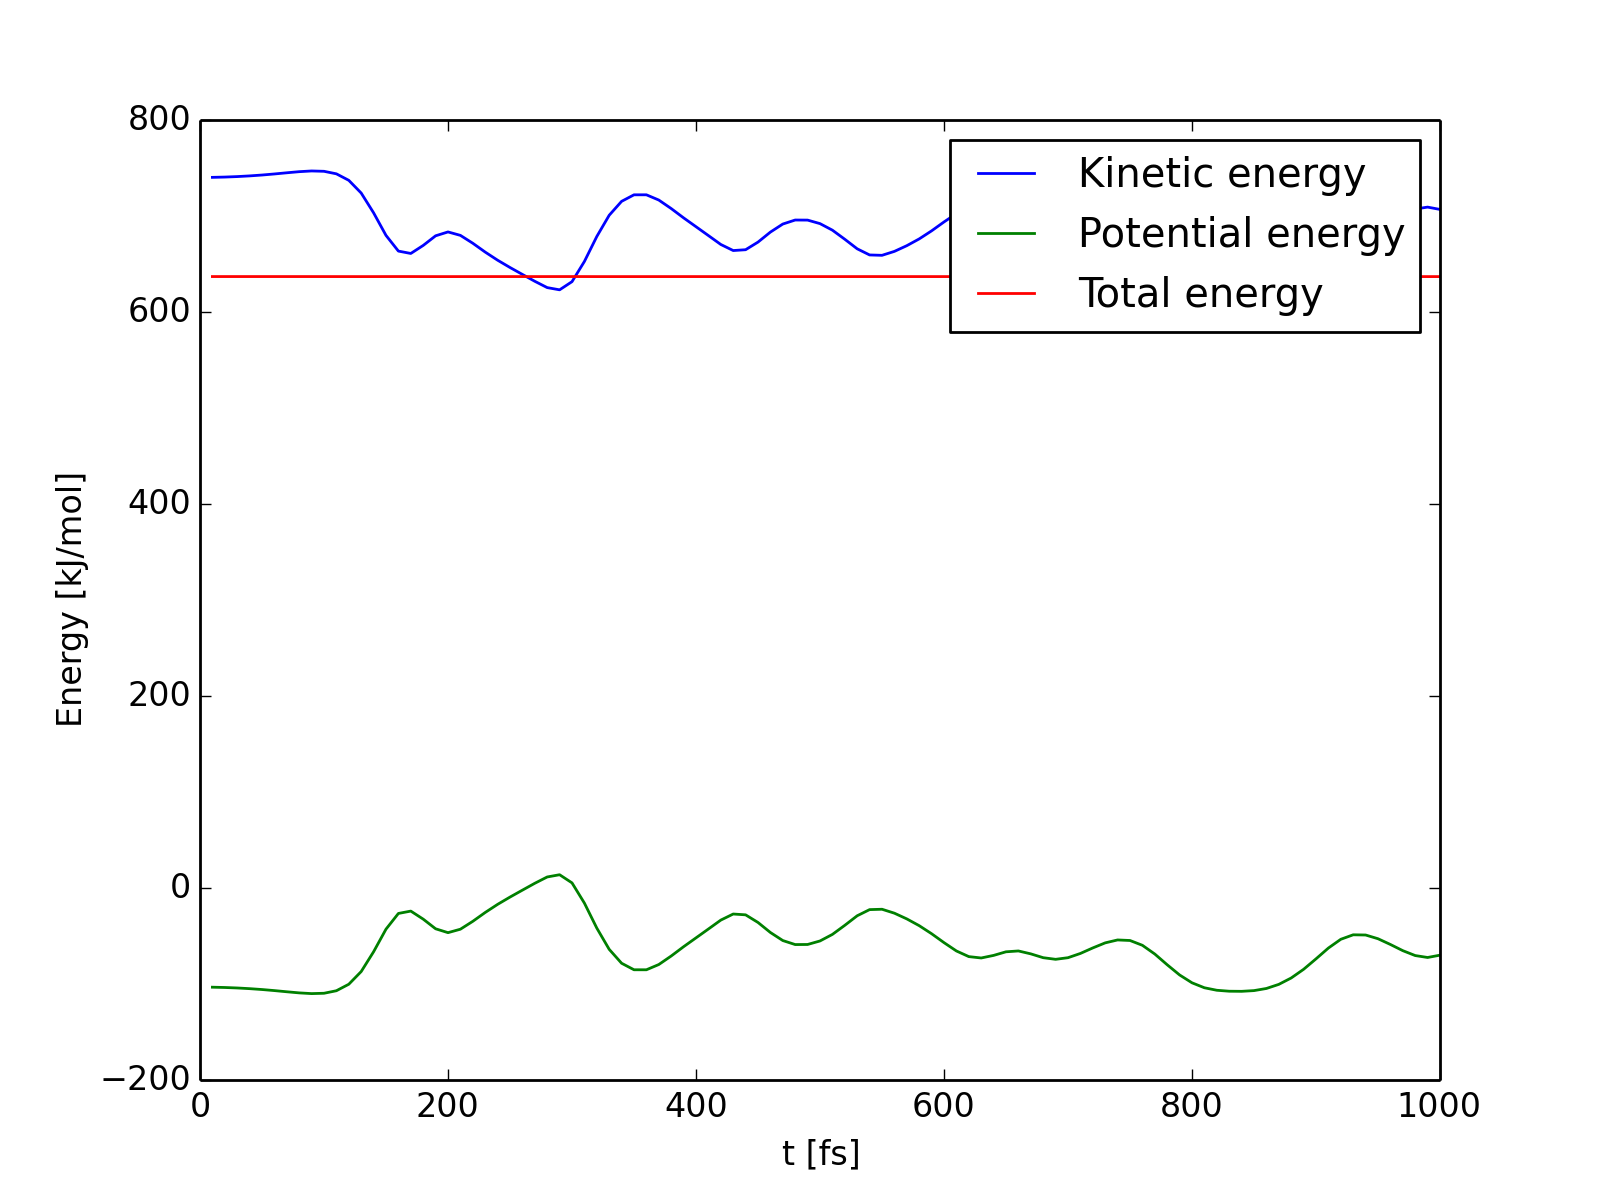
\includegraphics[width=0.75\textwidth]{images/energies}
    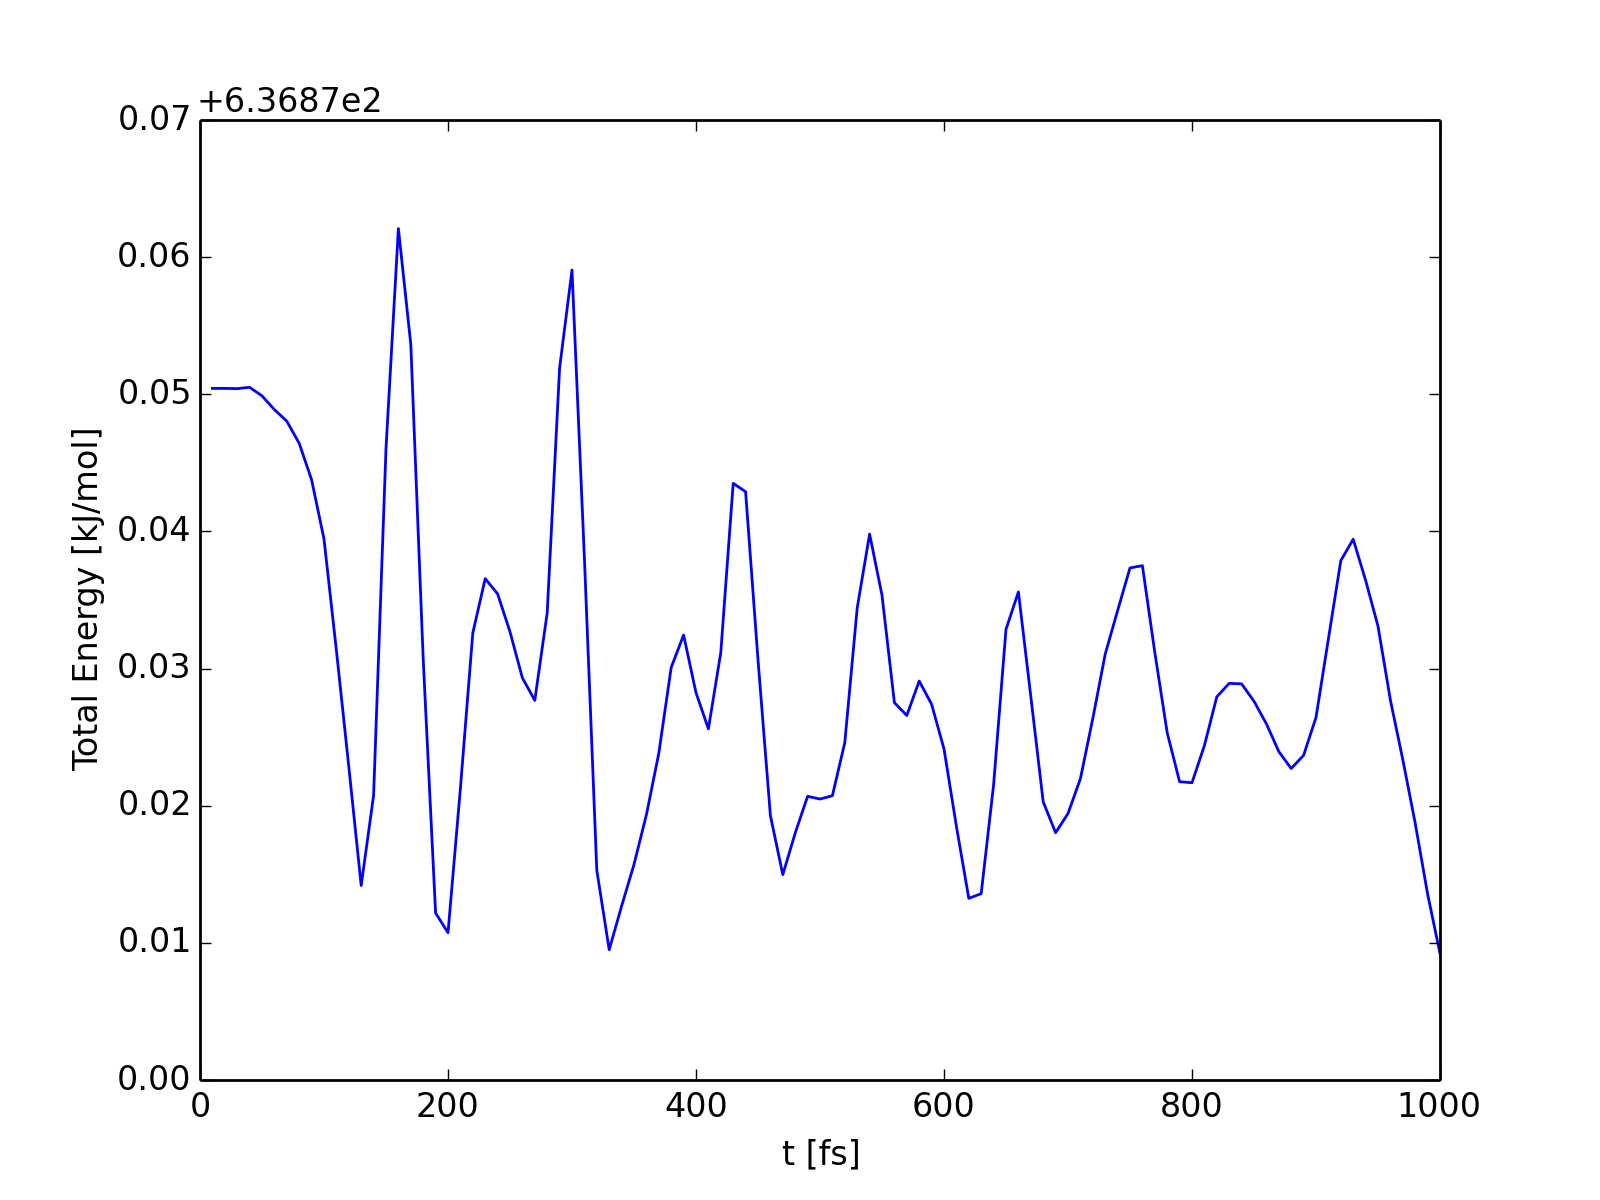
\includegraphics[width=0.46\textwidth]{images/etot}
    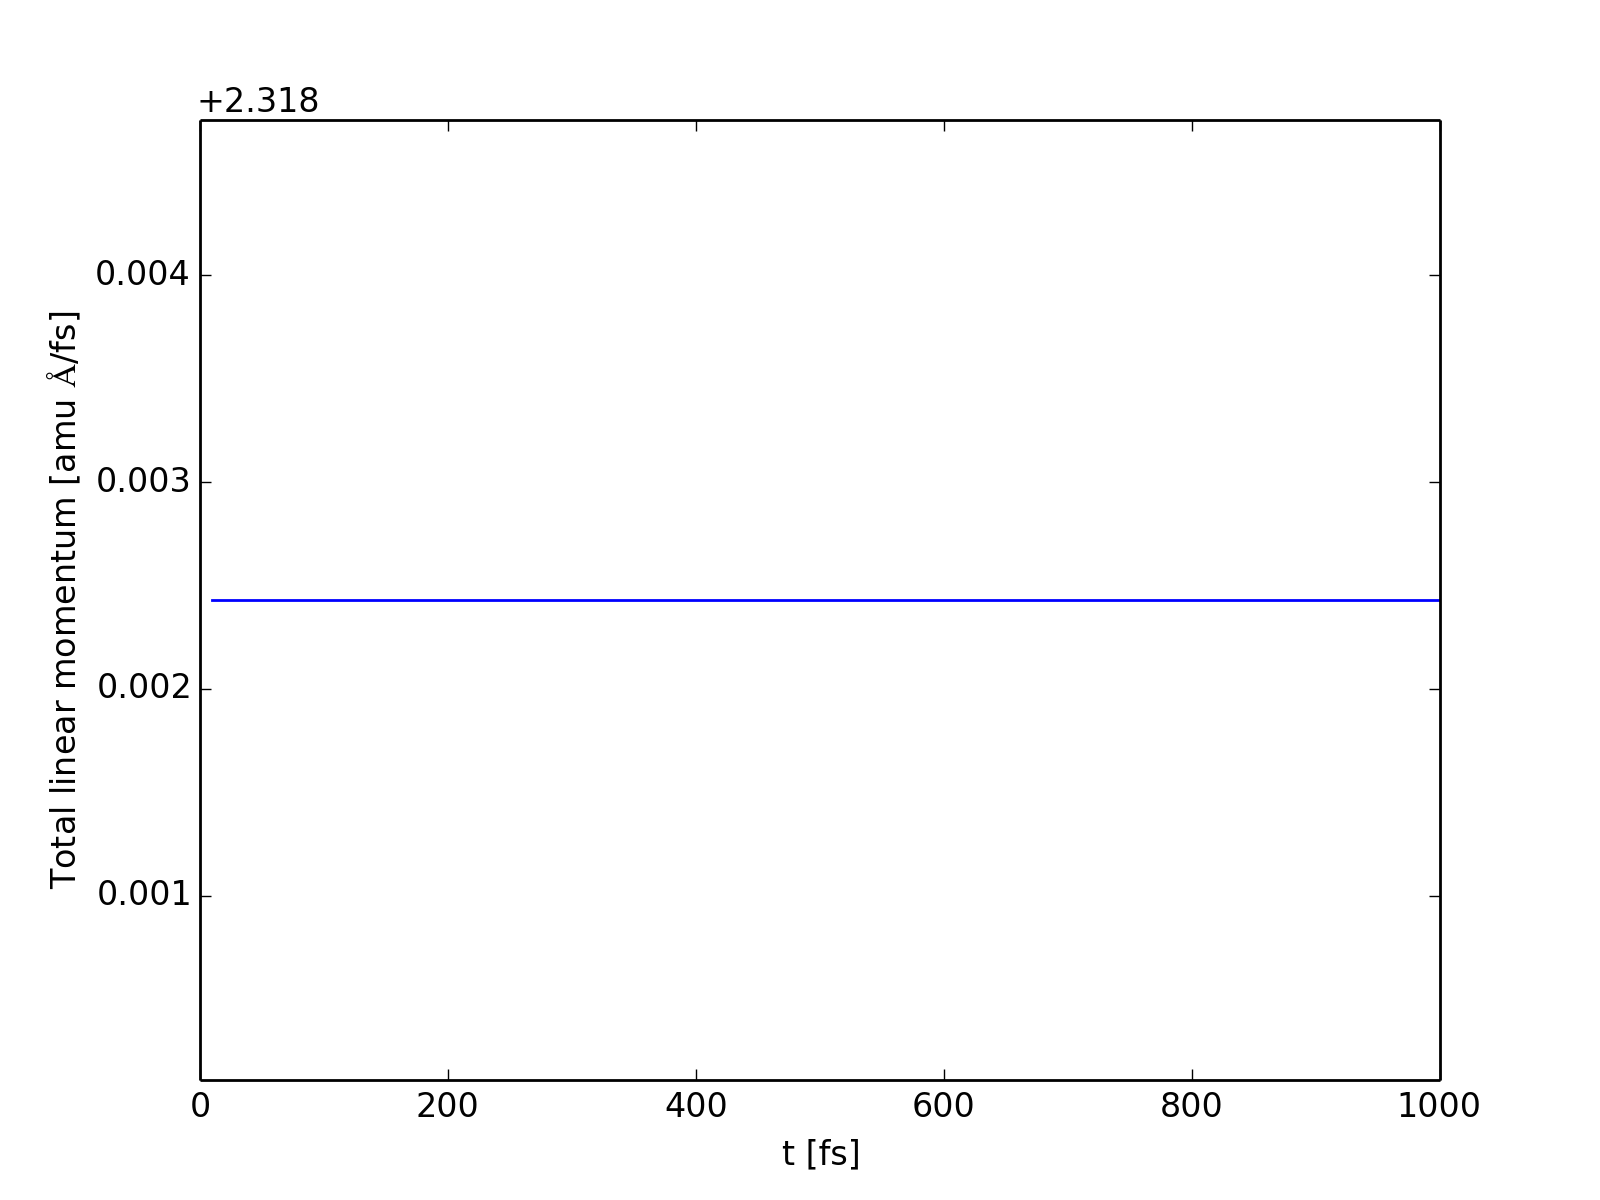
\includegraphics[width=0.46\textwidth]{images/ptot}
    \caption{Conserved quantities as a function of time.
             The simulation contains 125 argon atoms and is performed
             with a time step of 2fs.}
    \label{fig:cons}
\end{figure}

    For a problem size of $N=1000$, one integration step takes
    on average 6.86ms (see also Figure \ref{fig:scal}).
    At this problem size, the calculaltion of the forces already 
    dominates strongly, making up 99.5\% of the integration time.
    Obviously, Kernel 2 is the one that ought to be parallelized,
    with a possible speedup of up to 200x for $N=1000$.

\item Figure \ref{fig:scal} illustrates the scaling behavior of the CPU code,
    once compiled without optimization and once with optimization enabled.
    While optimization clearly speeds up the code drastically,
    the execution time of both versions is fitted well by a 2nd order 
    polynomial; the $N^2$ term of course dominating for large $N$.

\begin{figure}[h]
    \centering
    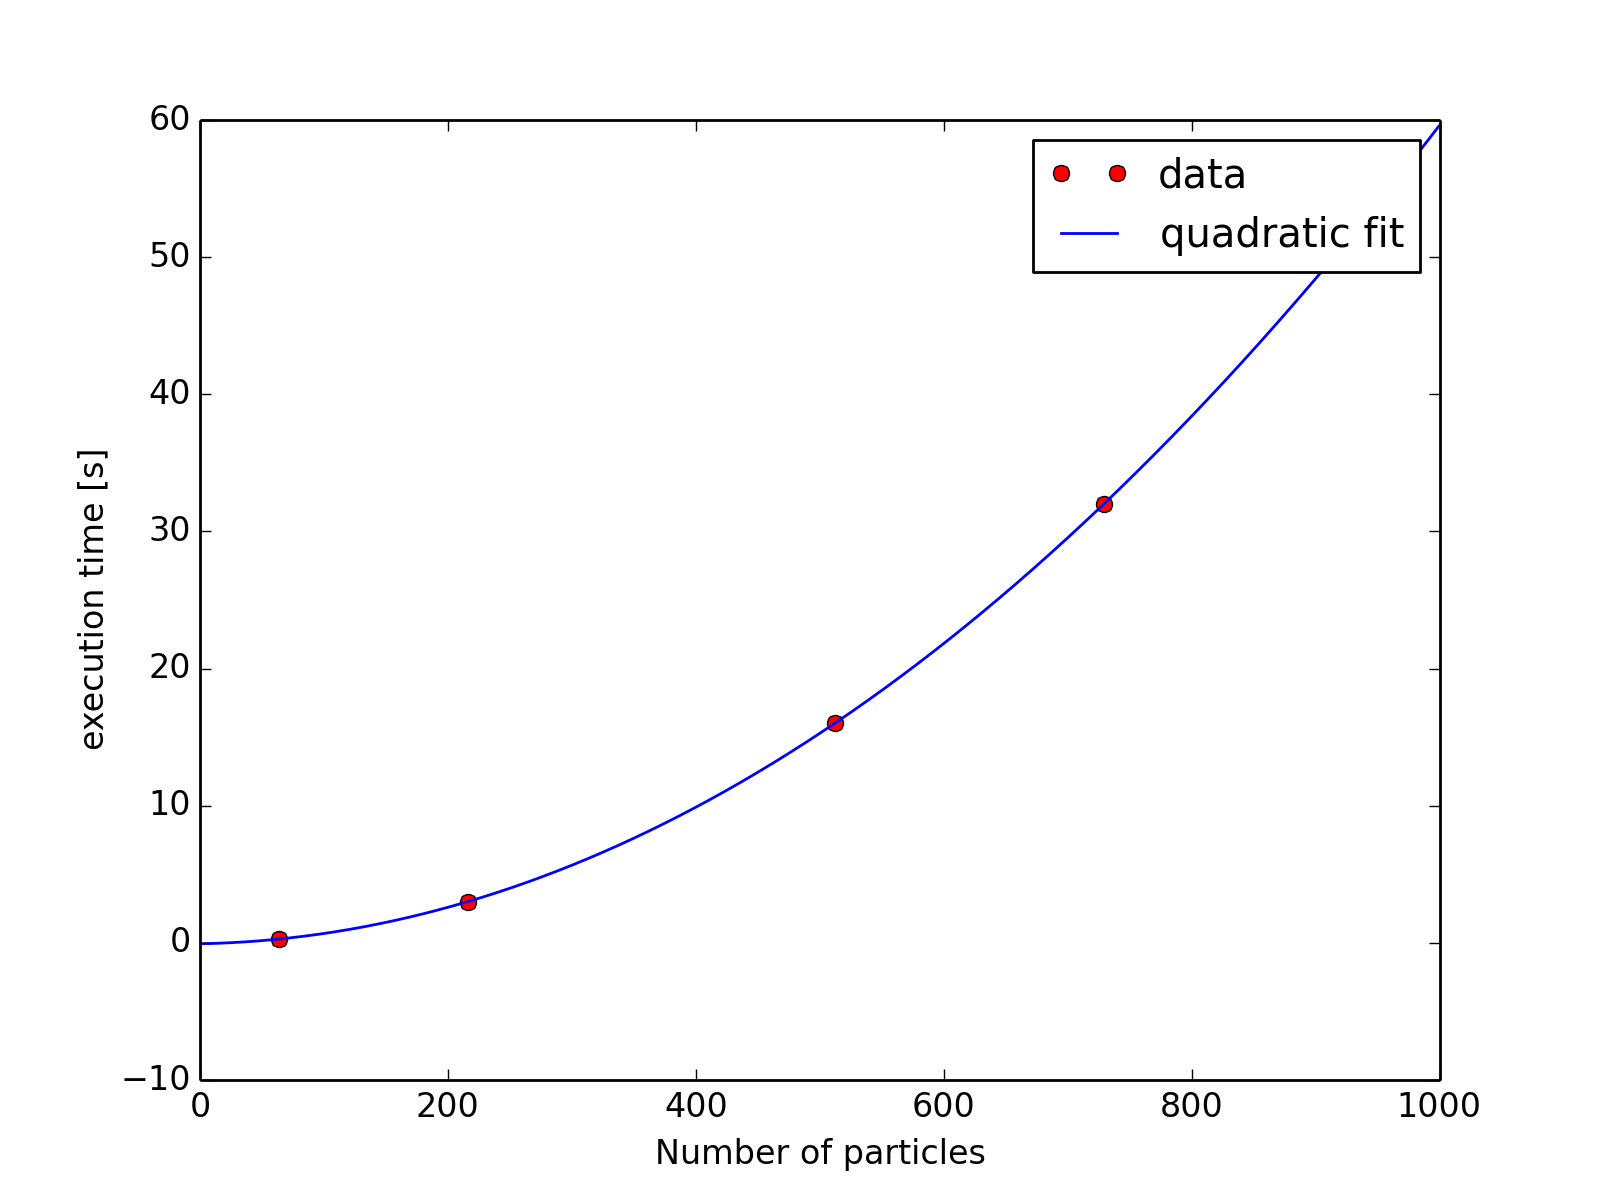
\includegraphics[width=0.80\textwidth]{images/scaling}
    \caption{Scaling of execution time versus problem size for a simulation
             time of 1ps (500 steps). 
             The calculations were performed on a single core of a Intel Core i7 
             processor with a clock frequency of 2.3 GHz and compiled with clang++.}
    \label{fig:scal}
\end{figure}

\end{enumerate}

\subsection{N-Body Problem on GPU}




%%%%%%%%%%%%%%%%%%%%%%%%%%%%%%%%%%%%%%%%%%%%%%%%%%%%%%%%%%%%%%%%%%
\section{Main structure of code \& details}

The two main tasks of an N-body solver are
\begin{enumerate}
    \item to calculate the forces for a given point in phase space and 
    \item to update the phase space coordinates using these forces.
\end{enumerate}

Since our solver should be able to treat different kinds of interactions,
the forces will be modularized. \verb|LennardJones| is a class derived
from a more general \verb|Force|  class.

Furthermore, we will need to compile the code on CPU and GPU architectures. 
We will use preprocessor instructions to swtich between the different
implementations for the different architectures (?).

\subsection{Appropriate data structure}
So, how would the optimal data structure look like?
The data sets that grow linearly with the number of particles $N$
are positions, velocities, forces and possibly neighbor lists%
\footnote{which may grow faster}, 
all of which are per-particle quantities.
It therefore seems reasonable to set up a
\verb|Particle| class, which is then instantiated as needed.

While this approach nicely groups the data,
there are performance drawbacks when compared to
storing each of these data sets in separate large arrays.

First, the data sets are not contiguous anymore.
This reduces cache efficiency in loops where only one 
dataset is required, e.g. the positions when building up
the neighbor lists.
Furthermore, we cannot make use of BLAS and LAPACK for efficient
vector and matrix operations. 
While the latter may be of great importance for other applications,
the operations performed by an N-body solver can typically not be recast
into standard linear algebra anyhow.
And finally, it may be detrimental to vectorization.

Second, $O(N)$ \verb|Particle| objects means $O(N)$ constructor
and destructor calls, which can be expensive in complex class trees.
In particular, virtual functions should be avoided.

All in all, it seems beneficial to abstain from 
grouping data in a \verb|Particle| class.
This still leaves the question of which containers to use.

\subsection{Appropriate containers}

When storing vectors and matrices, the tradeoff is between safety and
flexibility.

\begin{enumerate}
    \item \emph{The 'boxed' C++ way:} Using the safe and fast containers
        of the standard template library, 
        the Multiarray component of the \verb|boost| library
        or the \verb|thrust| library, which already aims at a host/device
        architecture.

        There are some drawbacks, however. 
        Since we aren't allowed to use C++11, intialization with STL containers
        is not very elegant. Using Multiarrays or thrust means adding a 
        library dependency.
    \item \emph{C-style arrays:} Clean syntax and flexibility 
        at the cost of reduced safety and having to take care of 
        memory management. This is certainly feasible and probably the 
        easiest solution.
    \item \emph{The C++ way:} Implementing the container yourself.
        This takes some extra time to code, but in the end offers a maximum of
        flexibility together with the possibility to make it safe and convenient.
\end{enumerate}

The only two non-standard containers required here are:
\begin{itemize}
    \item An $N$-dimensional vector of $3$-dimensional vectors to 
        store positions, velocities and forces.

        Within one such container, the coordinates should probably be grouped
        by particle and not by space direction. 
        It may be assumed that the number of particles $N$ remains constant
        in the course of the simulation.
        Helper functions to reset the container would be helpful.

        This can be achieved wihout problems by 1., 2. and 3.
        A vector of vectors may however break contiguity,
        since the 3d vectors would be allocated one-by-one.
        One should thus rely on a 2d array (2.) or a 1d vector (3.).

    \item An $N$-dimensional vector of lists with variable length
        to store the Verlet list of neighboring particles.

        The resizeable list is obviously a bit more tricky and strongly
        suggests to use \verb|std::list|, leaving options 1. and 3. 
        for this container.
\end{itemize}

\subsection{Parsing input}

Providing parameters via the command line works fine as long as there aren't
more than two or three.
An N-body solver with sensible flexibility needs more than that.
An minimalistic set of input parameters is listed in Table \ref{tab:input}.

\begin{table}
    \centering
\begin{tabular}[h!]{l|l}
    Symbol & Description \\\hline
    dt & time step \\
    t & total time \\
    nwrite & write info each x steps\\
    int & type of integrator\\
    fil\_xyz & .xyz file containing positions and atomic symbols\\
    temp0 & initial temperature\\ 
    f & the type of interaction\\
    lj\_sigma & Lennard-Jones $\sigma$ \\
    lj\_epsilon & Lennard-Jones $\varepsilon$\\
    lj\_rcut & Lennard-Jones cutoff radius\\
    cell\_x & cell size along x\\
    cell\_y & cell size along y\\
    cell\_z & cell size along z
\end{tabular}
    \caption{Input parameters for a calculation.}
    \label{tab:input}
\end{table}

We will therefore discard the provided \verb|ArgumentParser.h| and move
to the much more powerful \verb|boost::program_options|.

%%%%%%%%%%%%%%%%%%%%%%%%%%%%%%%%%%%%%%%%%%%%%%%%%%%%%%%%%%%%%%%%%%

\subsection{GPU - parallelization strategy}

In order to parallelize a single Lennard-Jones force update,
we need to

\begin{itemize}
    \item copy the positions from host to device,
    \item run the Lennard-Jones kernel on device, calculating the forces and
    \item copy forces back from device to host.
\end{itemize}

I.e. this requires transfer of O(N) data between CPU and GPU at every step.
The first question is therefore: Does this make sense or 
do we have to parallelize
the position \& velocity update as well and copy back to the host
only when required for a readout?

Assuming a data transfer rate of 9.6 GB/s and an array size of
24 KB for the positions of 1000 particles in double precision,
we arrive at 2.5$\mu$s transfer time, 
i.e. significantly smaller than the 40$\mu$s
for the non-LJ part for 1000 atoms.
For the latency, \href{http://www.princeton.edu/~dlustig/dlustig_HPCA13.pdf}{this benchmark}
reports values of the order of 10$\mu$s, i.e. quite low as well.

So, it \emph{does} make sense to parallelize a single force 
update step, although it would of course be faster
to parallelize more.


\subsection{GPU - data structures}

For the serial CPU version, it made sense to group data together that
belongs together conceptually, e.g. positions, velocities, forces and more
in a \verb|State| class.

For the GPU version we are confronted with the requirement to replicate
data on the GPU. And since the bandwidth is limited, we want to replicate only
as much as needed for the particular purpose.

It would seem sad to now start tearing apart the nice class structure,
just in order to save bandwidth.
There seems to be an acceptable intermediate solution: 
Make pointers out of class members that store significant amounts of data.
This adds the responsibility to deallocate the data behind the pointers,
but allows to copy the data behind these pointers to the GPU as needed.

Unfortunately, CUDA has no built-in mechanism for performing a 'deep copy'
between host and device.
One can accomplish \href{http://stackoverflow.com/questions/15431365/cudamemcpy-segmentation-fault/15435592#15435592}{deep copies manually},
but in this case one has to copy pointers and the data behind them
on a member-by-member basis.
This takes away much of the benefit from an object-oriented
design at the first place, 
results in a lot of ugly code and generally seems to be discouraged.

So, sadly, I don't see any alternative here to ugly code.
Calculating the Lennard-Jones forces is not a mere 'transformation' of
the position vector, so \verb|thrust| doesn't here and we have to 
write the kernel ourselves.

The only thing we can do is to make copying vectors from/to device
a bit easier, by providing member functions that do this.

\subsection{GPU - avoiding race conditions}


There is one particular problem that turns up in parallelizing
the force update. 
A standard serial implementation makes use of Newton's 3rd law
and thus for each pair of particles (i,j) updates the forces of both
particle i and j simultaneously.
When parallelizing over the index i,
this brings the danger of race conditions 
since every thread will, at some point in time, 
update the force on every particle.
There are several solutions to this problem:
\begin{itemize}
    \item neglect Newton's 3rd law, thus wasting 1/2 of computing time.
    \item having a private force array for each thread. 
        This doesn't seem practical, since it would require O($N^2$) memory.
    \item having two global copies of the force array.

        Each thread updates the force of particle i N times, but the forces of
        all other particles only once. One could therefore make the first
        In this scenario, each thread writes
    \item 
\end{itemize}<++>

\subsection{GPU - Load balacing}
When parallelizing the Lennard-Jones loop,
the loop over $i>j$ results in strongly unbalanced work packages.

Since our parallelization aims for $N\gg \#$ threads,
this is less of a problem as threads that are already finished
can 
Load balancing




\section{Source code}

Since the source code is spread over quite a few files,
I am not including it in the pdf file.
The source code is publicly available on
\url{https://github.com/leoteo/bounce}.

In order to clone the repository using the \href{http://git-scm.com}{Git} 
revision control system, do

\begin{verbatim}
git clone https://github.com/leoteo/bounce.git
\end{verbatim}

\end{document}
